\documentclass[border=1pt]{standalone}
% Shared preamble for standalone figures in this directory.
% Compile with XeLaTeX from 讲义/figs, or via the figures target.
\usepackage{ctex}
\usepackage{amsmath}
\usepackage{amssymb}
\usepackage{bm}
\usepackage{mathtools}
\usepackage{tikz}
\renewcommand{\vec}[1]{\boldsymbol{#1}}
\newcommand{\cC}{\mathcal{C}}
\newcommand{\cD}{\mathcal{D}}
\newcommand{\R}{\mathbf{R}}
\usetikzlibrary{
    arrows.meta,
    calc,
    decorations.markings,
    angles,
    quotes,
    positioning,
    patterns,
    shapes.geometric
}

\begin{document}
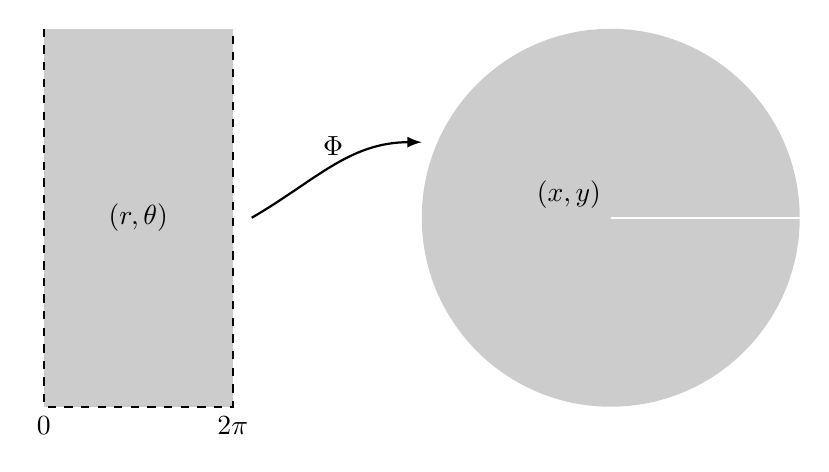
\begin{tikzpicture}[>=latex,scale=2.4]
    \fill[gray!40] (-0.5, -1) rectangle (0.5, 1);
    \draw[dashed, thick] (-0.5, 1) -- (-0.5, -1) node[below] {$0$} -- (0.5, -1) node[below] {$2\pi$} -- (0.5, 1);
    \fill[gray!40] (2.5, 0) circle (1);
    \draw[white, thick] (2.5, 0) -- (3.5, 0);
    \draw node at (0, 0) {$(r, \theta)$} node[above left] at (2.5, 0) {$(x, y)$};
    \draw[thick] (0.6, 0) edge[out=30, in=180, ->] node[above] {$\Phi$} (1.5, 0.4);
\end{tikzpicture}

\end{document}
